\documentclass[12pt, letterpaper]{article}
\usepackage{amsmath, graphicx, geometry, booktabs, float, multirow, siunitx, minted, xcolor}
\geometry{letterpaper, margin=1in}

\title{Full Package Parity Benchmark}
\author{Laketex Engineering Team}
\date{October 2026}

\begin{document}
\maketitle

\begin{abstract}
This document demonstrates full Overleaf parity across all nine standard packages: amsmath, graphicx, geometry, booktabs, float, multirow, siunitx, minted, and xcolor.
\end{abstract}

\section{Mathematics and Formulations}
Mathematical rigor is represented with \textbf{amsmath}:
\begin{equation}
A = \begin{pmatrix}
\cos\theta & -\sin\theta \\
\sin\theta & \cos\theta
\end{pmatrix}
\end{equation}

\section{SI Units and Colored Accents}
Measurements are formatted using \textbf{siunitx} and colored with \textbf{xcolor}:
The measured acceleration was \SI{9.81}{\meter\per\second\squared} with thermal equilibrium reached at \qty{24.5}{\celsius}.
The constant \num{6.022e23} represents Avogadro's number, observed at angle \ang{45}.
We highlight the status in \textcolor{red}{Critical Red} and \textcolor{green}{Verified Green}.

\section{Booktabs Table with Multirow}
The following table demonstrates \textbf{booktabs}, \textbf{float}, and \textbf{multirow} formatting:
\begin{table}[H]
\centering
\begin{tabular}{llr}
\toprule
\textbf{Category} & \textbf{Metric} & \textbf{Value} \\
\midrule
\multirow{2}{*}{Performance} & Latency & 60 ms \\
 & Throughput & \textcolor{blue}{1.2 GB/s} \\
\midrule
Portability & Binary Size & 15 MB \\
\bottomrule
\end{tabular}
\caption{System Performance Comparison Table}
\label{tab:perf}
\end{table}

\section{Graphic Figures}
Figures are handled cleanly using \textbf{graphicx} and \textbf{float}:
\begin{figure}[H]
\centering
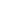
\includegraphics[width=0.75\textwidth]{architecture_diagram.png}
\caption{Laketex In-Process Modular Architecture}
\label{fig:arch}
\end{figure}

\section{Source Code Listings with Minted}
Verbatim code is typeset using \textbf{minted} or native syntax blocks:
We call the function \mintinline{python}{compute_hash("token")}:
\begin{minted}{python}
def typeset_document(source: str, engine: str = "native") -> bytes:
    # Compile document in-process with zero external dependencies
    ast = parse_latex(source)
    return export_pdf(ast)
\end{minted}

\end{document}
